\section*{Q3 [30 Marks]}

Apply DBSCAN with parameters MinPts = 4 and Eps = $\sqrt{2}$ to get clustering results.

\textbf{First}, for every data point, answer if it is a core, a border, or an outlier. \\
\textbf{Second}, for data points that are not outliers, show the clusters detected. \\
\textbf{Third}, show your detailed steps of DBSCAN process, including the content of the queue you maintain, whenever a new core is found.

\begin{center}
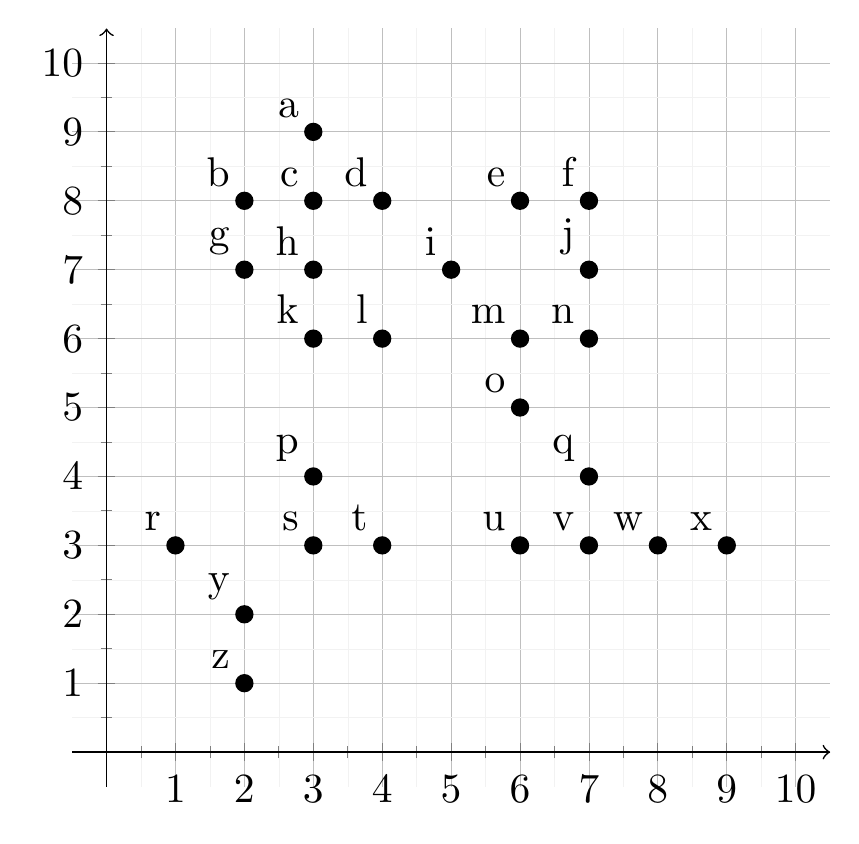
\begin{tikzpicture}[scale=1.5]
    \begin{axis}[
        width=8cm, % Set the width of the grid
        height=8cm, % Set the height of the grid
        xmin=0, xmax=10,
        ymin=0, ymax=10,
        axis lines=center,
        axis line style={->},
        xlabel={},
        ylabel={},
        grid=both,
        grid style={line width=.1pt, draw=gray!10},
        major grid style={line width=.2pt,draw=gray!50},
        xtick={0,1,...,10},
        ytick={0,1,...,10},
        minor tick num=1,
        enlargelimits={abs=0.5},
        axis equal image=true,
        scatter/classes={
            a={mark=*,draw=black,fill=black,scale=1}
        }
        ]

        % Add points here
        \addplot[scatter,only marks,scatter src=explicit symbolic]
        table[meta=label] {
        x     y     label
        3     9     a
        2     8     a
        3     8     a
        4     8     a
        6     8     a
        7     8     a
        2     7     a
        3     7     a
        5     7     a
        7     7     a
        3     6     a
        4     6     a
        6     6     a
        7     6     a
        6     5     a
        3     4     a
        7     4     a
        1     3     a
        3     3     a
        4     3     a
        6     3     a
        7     3     a
        8     3     a
        9     3     a
        2     2     a
        2     1     a
        };

        \node[above left] at (axis cs:3,9) {a};
        \node[above left] at (axis cs:2,8) {b};
        \node[above left] at (axis cs:3,8) {c};
        \node[above left] at (axis cs:4,8) {d};
        \node[above left] at (axis cs:6,8) {e};
        \node[above left] at (axis cs:7,8) {f};
        \node[above left] at (axis cs:2,7) {g};
        \node[above left] at (axis cs:3,7) {h};
        \node[above left] at (axis cs:5,7) {i};
        \node[above left] at (axis cs:7,7) {j};
        \node[above left] at (axis cs:3,6) {k};
        \node[above left] at (axis cs:4,6) {l};
        \node[above left] at (axis cs:6,6) {m};
        \node[above left] at (axis cs:7,6) {n};
        \node[above left] at (axis cs:6,5) {o};
        \node[above left] at (axis cs:3,4) {p};
        \node[above left] at (axis cs:7,4) {q};
        \node[above left] at (axis cs:1,3) {r};
        \node[above left] at (axis cs:3,3) {s};
        \node[above left] at (axis cs:4,3) {t};
        \node[above left] at (axis cs:6,3) {u};
        \node[above left] at (axis cs:7,3) {v};
        \node[above left] at (axis cs:8,3) {w};
        \node[above left] at (axis cs:9,3) {x};
        \node[above left] at (axis cs:2,2) {y};
        \node[above left] at (axis cs:2,1) {z};
    \end{axis}
\end{tikzpicture}
\end{center}

\subsection*{Solution:}

If the size of N(p) is at least 4, then p is a core point. \\
We can find:

\begin{table}[h]
    \centering
    \begin{tabular}{@{}|c|c|c|c|@{}}
        \hline
        Point & N(p) & Point & N(p)   \\
        \hline
        a & \{a,b,c,d\} & n & \{j,m,n,o\} \\
        \hline
        b & \{a,b,c,g,h\} & o & \{m,n,o,q\} \\
        \hline
        c & \{a,b,c,d,g,h\} & p & \{p,s,t\} \\
        \hline
        d & \{a,c,d,h\} & q & \{o,q,u,v,w\} \\
        \hline
        e & \{e,f,i,j\} & r & \{r,y\} \\
        \hline
        f & \{e,f,j\} & s & \{p,s,t,y\} \\
        \hline
        g & \{b,c,g,h,k\} & t & \{p,s,t\} \\
        \hline
        h & \{b,c,d,g,h,k,l\} & u & \{q,u,v\} \\
        \hline
        i & \{d,e,i,m\} & v & \{q,u,v,w\} \\
        \hline
        j & \{e,f,j,m,n\} & w & \{q,v,w,x\} \\
        \hline
        k & \{g,h,k,l\} & x & \{w,x\} \\
        \hline
        l & \{h,i,k,l\} & y & \{r,s,y,z\} \\
        \hline
        m & \{i,j,m,n,o\} & z & \{y,z\} \\
        \hline
    \end{tabular}
\end{table}

We find that points a, b, c, d, e, g, h, i, j, k, l, m, n, o, q, s, v, w, y are core points. \\
The other points are border points. \\
And there are no outliers.

\begin{center}
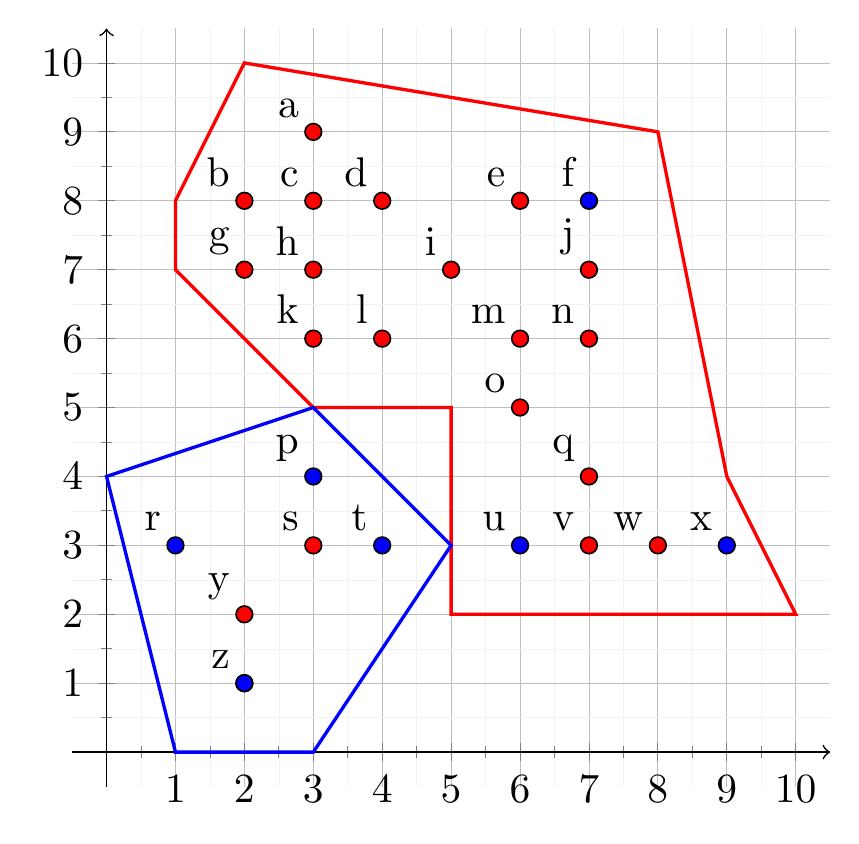
\begin{tikzpicture}[scale=1.5]
    \begin{axis}[
        width=8cm, % Set the width of the grid
        height=8cm, % Set the height of the grid
        xmin=0, xmax=10,
        ymin=0, ymax=10,
        axis lines=center,
        axis line style={->},
        xlabel={},
        ylabel={},
        grid=both,
        grid style={line width=.1pt, draw=gray!10},
        major grid style={line width=.2pt,draw=gray!50},
        xtick={0,1,...,10},
        ytick={0,1,...,10},
        minor tick num=1,
        enlargelimits={abs=0.5},
        axis equal image=true,
        scatter/classes={
            a={mark=*,draw=black,fill=black,scale=1}
        }
        ]

        % Add points here
        \addplot[only marks, mark=*,mark options={fill=red}]
        table[meta=label] {
        x     y     label
        3     9     a
        2     8     a
        3     8     a
        4     8     a
        6     8     a
        2     7     a
        3     7     a
        5     7     a
        7     7     a
        3     6     a
        4     6     a
        6     6     a
        7     6     a
        6     5     a
        7     4     a
        3     3     a
        7     3     a
        8     3     a
        2     2     a
        2     1     a
        };

        \addplot[only marks, mark=*,mark options={fill=blue}]
        table[meta=label] {
        x     y     label
        7     8     a
        3     4     a
        1     3     a
        4     3     a
        6     3     a
        9     3     a
        2     1     a
        };

        \node[above left] at (axis cs:3,9) {a};
        \node[above left] at (axis cs:2,8) {b};
        \node[above left] at (axis cs:3,8) {c};
        \node[above left] at (axis cs:4,8) {d};
        \node[above left] at (axis cs:6,8) {e};
        \node[above left] at (axis cs:7,8) {f};
        \node[above left] at (axis cs:2,7) {g};
        \node[above left] at (axis cs:3,7) {h};
        \node[above left] at (axis cs:5,7) {i};
        \node[above left] at (axis cs:7,7) {j};
        \node[above left] at (axis cs:3,6) {k};
        \node[above left] at (axis cs:4,6) {l};
        \node[above left] at (axis cs:6,6) {m};
        \node[above left] at (axis cs:7,6) {n};
        \node[above left] at (axis cs:6,5) {o};
        \node[above left] at (axis cs:3,4) {p};
        \node[above left] at (axis cs:7,4) {q};
        \node[above left] at (axis cs:1,3) {r};
        \node[above left] at (axis cs:3,3) {s};
        \node[above left] at (axis cs:4,3) {t};
        \node[above left] at (axis cs:6,3) {u};
        \node[above left] at (axis cs:7,3) {v};
        \node[above left] at (axis cs:8,3) {w};
        \node[above left] at (axis cs:9,3) {x};
        \node[above left] at (axis cs:2,2) {y};
        \node[above left] at (axis cs:2,1) {z};

        \draw[red, thick] (axis cs:2,10) -- (axis cs:1,8) -- (axis cs:1,7) -- (axis cs:3,5) -- (axis cs:5,5) -- (axis cs:5,2) -- (axis cs:10,2) -- (axis cs:9,4) -- (axis cs:8,9) -- cycle;
        \draw[blue, thick] (axis cs:3,5) -- (axis cs:5,3) -- (axis cs:3,0) -- (axis cs:1,0) -- (axis cs:0,4) -- cycle;
    \end{axis}
\end{tikzpicture}
\end{center}

In the scatter plot below, the red points are core points, the blue points are border points, and the green points are outliers (which actually do not exist). \\
And we detect 2 clusters which are circled in red and blue frames.